\section{Введение}
\subsection{Актуальность работы}

Кровь -- соединительная ткань внутри организма, она состоит из форменных клеток (эритроцитов, лейкоцитов, тромбоцитов), а так же из
водного раствора белков и свёртывающих веществ -- плазмы. Кровь под воздействием периодических сокращений сердечной мышцы 
движется по замкнутой системе сосудов, циркулируя от сердца и обратно. С точки зрения гидродинамики кровоток представляет 
из себя пульсирующее с низкой частотой течение мелкодисперсной суспензии в 
замкнутой системе каналов кругового сечения с эластичными стенками, осложнённое локальными эффектами ламинарно-турбулентного перехода.

Кровь, двигаясь по сосудам, испытывает сопротивление движению со стороны сосудов и из-за своей вязкости. Поэтому сердце вбрасывает 
кровь в сосуды под большим давлением. В аорте давление колеблется в диапазоне от 16~кПа при систоле до 10~кПа при диастоле. 
По мере движения крови давление в сосудистом русле падает. 
Скорость течения крови так же зависит от диаметра сосуда, удалённости сосуда от сердца, а также фазы сердечного цикла. 
Максимальных значений скорость достигает в аорте (до \texttilde$1$~м/с), а минимальных -- в капиллярах (около нуля).

Сложность разветвления кровеносных сосудов и вариации их размеров создают значительные трудности при решении задачи о течении крови. 
Математическое моделирование помогает  
пониманию сложностей кровотока. Эти модели позволяют описывать и строить физические процессы, происходящие 
в биологических системах. Это может быть полезно при выявлении, прогрессировании и лечении  различных сердечно-сосудистых заболеваний , 
а так же в проектировании и оптимизации медицинских устройств.

Кровь состоит из взвешенных в плазме 
(её рассматривают, как ньютоновскую жидкость) клеток крови, которые действуют друг на друга с некоторыми силами. 
Самые детальные методы моделирования заключаются в построении модели течения этих клеток как отдельных частиц в вязкой жидкости.
Описание такого типа методов можно подробнее изучить в ~\cite{Fedosov:2010,Fedosov:2008,Mehboudi:2001}. 
В некоторых моделях ~\cite{bessonov:2014,hosseini:2009} пренебрегают относительно мелкими и редкими -- тромбоцитами
(2--4~мкм в количестве 150--300 миллионов на 1~см$^3$) и лейкоцитами(4--20~мкм в количестве 4.5 -- 11 миллионов на 1~см$^3$), 
а моделируют лишь самые крупные из них -- эритроциты (7 -- 8~мкм в количестве 3.8 до 5.6 миллиардов клеток на 1~см$^3$).
Метод ресурсоёмкий, поэтому можно моделировать лишь небольшие участки кровотока (порядка 1~см и меньше) без ветвлений 
либо с одним - двумя ветвлениями.
Так же такая модель плохо реагирует на любые изменения в исходных данных, ведь свойства эритроцитов могут значительно изменяться, 
а модель строится под определённую их конфигурацию~\cite{Yamaguchi2010}. 
Соответсвенно, возникает необходимость прибегнуть к некоторым упрощениям постановки.

Можно не описывать индивидуальные частицы взвешенные в плазме, а обобщить их до вязкой неньютоновской жидкости с определёнными 
характеристиками, в которых отразить эффекты, связанные с наличием взвешенных в растворе частиц. Такой подход называют трехмерным моделированием.
Принципиальным моментом в формулировке такой постановки является выбор модели вязкости: например,
основанные на зависимости вязкости от гематокрита ~\cite{walburn:1976},
модель Максвелла \cite{thurston:1972},  модель Кассона ~\cite{moller:2006}.
Однако эти модели всё-таки требуют значительных вычислительных ресурсов, поэтому имеет смысл провести дальнейшее упрощение.

Наиболее простыми с точки зрения вычислительных ресурсов являются так называемые одномерные модели кровотока, в которых
пространственные характеристики осредняются по поперечному сечению, а трёхмерная дифференциальная
задача сводится к одномерной.

В некоторых случаях эти модели используют для постановки граничных условий в многомерных задачах. (ссыдки)
Но так же они могут и целиком моделировать кровеносную систему.(ссылки)

Такой подход к моделированию требует меньших вычислительных ресурсов, но при этом почти не уступает в 
точности другим моделям. О сравнении одномерных и многомерных моделей можно прочитать в ~\cite{FORMAGGIA:2001}.

{\bfВывод об актуальности}
Таким образом, несмотря на значительное увеличение доступных вычислительных мощностей и активное развитие детальных методов
численного моделирования гемодинамики, до сих пор полное описание системы кровообращения подробными моделями остаётся невозможным, 
а прямое или косвенное использование одномерных моделей для таких задач является безальтернативным выбором.
Поэтому развитие таких упрощённых моделей является актуальной задачей

\subsection{Обзор методов моделирования на основе одномерной постановки}

Принципиальным вопросом в построении одномерной модели кровотока является выбор зависимости давления в сосуде от площади его
поперечного сечения.

Можно использовать $N$ интегральных условий сохранения Бернулли выражающих непрерывность полного давления $P^l$:
\begin{equation}
    \label{eq:bernulli}
    \frac{\rho u^2_k}{2}+{p_k(A_k)}=P^l.
\end{equation}
Иногда для моделирования сопротивления потоку в местах стыка используют условия перепада давлений
с учётом сопротивления
\begin{equation}
    \label{eq:p-pressure}
    p_k\left(A_k\left(t,x_k\right)\right)-p^l(t)=\varepsilon_k R^l_k A_k(t,x_k)u_k(t,x_k),
\end{equation}
которое выражается через коэффициент $R^l_k$. Здесь $p^l$ -- давление в точке бифуркации \cite{bessonov:2014}.

Но общим способом замыкания системы является явное представление алгебраической зависимости
между давлением в сосуде и его площадью. Прямой подход к получению отношения $p(A)$ включает в себя точное одновременное измерение
давления и площади в разные моменты времени. Но такой метод не всегда удобен в реальности.
Качественный анализ физических экспериментов подтверждает, что функция $p(A)$ должна быть монотонной S-подобной кривой. 
Такая кривая удовлетворительно описывает состояния как круглого, так и эллиптического сечения. На рис.~\ref{ych} показана зависимость
зависимость давления в сосуде от его площади.


\begin{figure}[h]
    \centering
    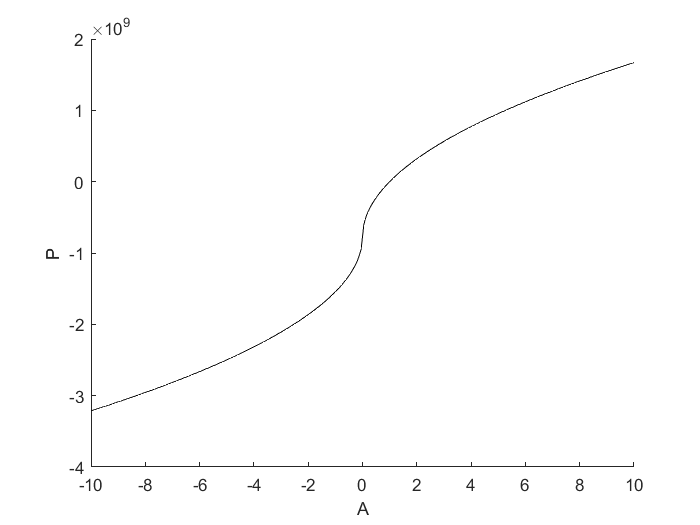
\includegraphics[width=0.6\linewidth]{PA.png}
    \caption{График зависимости давления от поперечного сечения внутри сосуда.}
    \label{ych}
\end{figure}

Для решения дифференциальных уравнений нужно выбрать подходящий метод.

Метод конечных разностей предполагает дискретизацию области на сетку точек и последующую аппроксимацию производных в управляющих
уравнениях с помощью конечных разностей. Этот метод часто используется в сочетании со схемой интегрирования по времени для решения 
полученной системы обыкновенных дифференциальных уравнений.

Метод конечных элементов~\cite{TAYLOR1998} -- популярная численная схема. 
Он особенно хорошо подходит для моделирования сложных геометрий, таких как запутанная сеть артерий в человеческом теле. 
Однако он может быть вычислительно дорогим, особенно для больших и сильно разветвленных сетей. 

Метод быстрого преобразования Фурье~\cite{Sazonov:2019} -- 
это подход, использующий быстрое преобразование Фурье для решения одномерных уравнений кровотока. 
Этот метод конкурирует с традиционными пространственно-временными численными схемами как по устойчивости, так и по скорости. 
Он может точно и эффективно обрабатывать сложные геометрические формы и высокоамплитудные волны. 
Однако он требует дальнейшего развития для учета вязкоупругих эффектов и потери массы крови из-за мелких ветвей. 

Метод прерывистого Галеркина~\cite{yao:2017} -- это еще одна численная схема, она сочетает в себе преимущества методов конечной разности и конечных элементов, 
обеспечивая баланс между точностью и вычислительными затратами. Однако он может быть более сложным в реализации и может
потребовать дополнительных вычислительных ресурсов для сопоставления расчетной и физической областей.

Метод конечных объемов с локальным временным шагом высокого порядка~\cite{mueller:2015} предполагает решение управляющих уравнений 
с помощью метода конечных объемов высокого порядка и схемы локального шага по времени. 
Этот метод может быть особенно полезен для моделирования течения в сложных геометрических системах.


Об источнке:
1) какой процесс исследовали, цель
2) использовали p(a) или метод аппроксисмации.
3) Может быть там есть сравнение интерисующих вас деталей.



\section{Постановка задачи}
2) граничные условия

Обосновать условия состыковки
Область расчёта.

По второму закону Ньютона движение среды определяется действием массовых и поверхностных сил. 
Законы сохранения массы и импульса для сплошной среды могут быть
записаны в переменных $(A, u, p)$: 
\begin{align}
    \label{eq:mass-balance}
    \varphi=&\frac{\partial A}{\partial t}+\frac{\partial Au}{\partial x},\\
    \label{eq:momentum-balance}
    \psi=&\frac{\partial u}{\partial t}+ \frac{\partial u^2/2+p/\rho}{\partial x}
\end{align}
Здесь $t$ -- время, $x$ -- координата вдоль сосуда, $A(t, x)$ -- площадь поперечного сечения сосуда, 
$u(t, x)$ и $p$ -- усредненная по сечению линейная скорость и трансмуральное давление крови. 

В системе три неизвестных: $(A, u, p)$, поэтому в каждой конечной точке сосуда требуется одно дополнительное условие совместимости.
Например, сохранение массы:
\begin{equation}
    \label{eq:conserv-mass}
    \sum_{k=k_1,k_2,...,k_N} \varepsilon_k A_k(t,x_k)u_k(t,x_k)=0,
\end{equation}
где {$k_1,...,k_N$} -- индексы сосудов, $\varepsilon_k=1, x_k=0$ -- для входящих сосудов,
$\varepsilon_k=1, x_k=L_k$ -- для выходящих сосудов.

Или же, одну из описанных выше, зависимостей давления в сосуде от площади поперечного сечения.

Рассмотрим систему уравнений, описывающую кровоток в одиночном сосуде (\ref{eq:mass-balance}) -- (\ref{eq:momentum-balance}) при условии
отсутствия источников/стоков ($\varphi=0$).
Из внешних сил, действующих на поток будем учитывать силу трения.
Для этого зададимся профилем скорости согласно \cite{smith:2002}:
$$
\tilde u(x, \xi) = u(x) \frac{\zeta + 2}{\zeta} \left[1 - \left(\frac{\xi}{r}\right)^\zeta\right],
$$
где $r$ -- радиус скругления, $\xi$ -- радиальная координата, $\zeta$ -- константа, определяющая профиль.
В результате интегрирования уравнений Навье-Стокса получим значение силы трения (см. \cite{boileau:2015}):

$$
\psi = -\frac{2 (\zeta + 2) \mu \pi u}{\rho A}.
$$

Запишем определяющую систему уравнений в виде

\begin{equation*}
    %\label{sys_of_eq}
    \begin{cases}
	&\dfrac{\partial A}{\partial t}+\dfrac{\partial Au}{\partial x}=0,\\[10pt]
	&\dfrac{\partial u}{\partial t}+u\dfrac{\partial u}{\partial x}+\dfrac{1}{\rho}\dfrac{\partial p}{\partial x}=\psi(u, A),\\[10pt]
	&p=\dfrac{4}{3}\sqrt{\pi}\dfrac{Eh}{A_0}(\sqrt{A}-\sqrt{A_0}).
    \end{cases}
\end{equation*}
Здесь использована замыкающая зависимость $p(A)$ из работы \cite{boileau:2015}, учитывающая
эластичные свойства стенок сосудов через параметры $E$ -- модуль упругости и $h$ -- толщина стенок сосуда.

Проведём обезразмеривание системы:
\begin{equation}
    \label{sys_of_eq1}
    \begin{cases}
	\dfrac{\partial A}{\partial t}+\dfrac{\partial Au}{\partial x}=0,\\[10pt]
	\dfrac{\partial u}{\partial t}+\dfrac{1}{2}\dfrac{\partial u^2}{\partial x} = -\dfrac{\partial p}{\partial x}-M_f \dfrac{u}{A},\\[10pt]
	p=M_p(\sqrt{A}-1).
    \end{cases}
    \end{equation}
В результате все физические параметры задачи определены через два безразмерных комплекса
$$
M_f=\frac{2(\zeta+2)\mu \pi L}{\rho A_0 U_0}, \quad
M_p=\frac{4\sqrt{\pi}Eh}{3 \rho U_0^2\sqrt{A_0}},
$$
где $L$ -- характерная длина сосуда, $A_0$ -- характерная площадь поперечного сечения сосуда, $U_0$ -- характерная скорость потока.
Первое из них описывает трение жидкости о стенки сосуда, второе -- эластичные свойства стенок сосуда.
Характерное время процесса при этом определится как $t_0 = L/U_0$.

Определяющая система дифференциальных уравнений (\ref{sys_of_eq1}) включает в себя два гиперболических уравнения.
Первое из них имеет вид уравнения переноса, второе -- уравнения Бюргерса.

Для одномерных моделей кровотока необходимы граничные условия на стыках сосудов, входах и выходах в сети сосудов.
Для всех сосудов граничные условия должны включать условия совместимости по характеристикам системы гиперболических уравнений (\ref{eq:mass-balance}), (\ref{eq:momentum-balance})~\cite{Xiu:2007}.
В каждой конечной точке сосуда требуется только одно дополнительное условие совместимости.
Вторым условным граничным условием на стыке N сосудов является сохранение массы:
\begin{equation}
    \label{eq:conserv-mass}
    \sum_{k=k_1,k_2,...,k_N} \varepsilon_k A_k(t,x_k)u_k(t,x_k)=0,
\end{equation}
где {$k_1,...,k_N$} -- индексы сосудов, $\varepsilon_k=1, x_k=0$ -- для входящих сосудов,
$\varepsilon_k=1, x_k=L_k$ -- для выходящих сосудов.

Выходы сети артерий и входы сети вен должны быть связаны с множеством мелких неучтенных сосудов, относящихся к микрососудистым регионам.
Поток в таких сосудах не может быть описан одномерными моделями течения (\ref{eq:mass-balance})-(\ref{eq:mass-conserv})
из-за большого количества сосудов, сложной структуры микрососудистых сетей и неньютоновской реологии крови.

Более простой подход заключается в том, чтобы объединить артерий и вены в точки соединения,
где выполняются (\ref{eq:conserv-mass}),(\ref{eq:p-pressure}). Коэффициенты сопротивления $ R^l_k$ оцениваются  по известному перепаду
давления между артериями и венами. Чем больше сосудистая сеть, тем меньше сосудов объединяются, тем выше точность метода.
Более подходящие граничные условия оттока: отдельные участки мелких артерий и микроциркуляции моделируются как структурированные деревья,
чей импеданс корней может быть оценен из линеаризации управляющих уравнений.

Некоторые авторы~\cite{alastruey:2008} выполняют сопряжение во временной области 1D моделей кровотока с электрическими цепями
(единичными параметрами) 0D моделей. 0D модели обеспечивают корректные граничные условия для глобальных моделей кровотока.


Вычислительной областью модели является сосудистая одномерная сеть или же её части. Сеть создаётся на основе общих анатомических данных,
например, справочник анатомических карт ~\cite{bunicheva:2013}, анатомические 3D модели или данные конкретного человека или животного. 
Задаётся так же и физические характеристики крови, такие как плотность: обычно её оценивают в 1052 -- 1060~кг/м\textsuperscript{3},
вязкость (4.3 -- 4.9~мПа$\cdot$). 



\section{Метод решения}
